\section{Kalibrierung des Szintillators}

\subsection{Vergleich der Detektorspektren}

Im ersten Schritt wurden die Spektren mehrerer Quellen für den Szintillator, wie auch den Ge-Detektor, aufgenommen und die Ergebnisse verglichen.
Genutzt wurden hierfür eine $^{22}$Na und eine $^{133}$Ba Probe, welche auf den Ge-Detektor und neben den Szintillator gelegt wurden.
Die Messzeit betrug für $^{22}$Na 5 min und für $^{133}$Ba 4min.
Eine Messung der Untergrundstrahlung wurde nicht durchgeführt, da sie für den einfachen Vergleich zweier Spektren auch nicht notwendig wäre.
Wie in Abb. \ref{NaGe} und \ref{NaSzin} zu sehen ist, war die Aktivität der $^{22}$Na Probe recht niedrig.
Im Ge-Spektrum lässt sich prinzipiel ein stark ausgeprägter Peak, zwischen den Kanälen 500 und 600, erkennen, das Compton-Kontinuum ist jedoch recht verschwommen.
Das Szintillator-Spektrum wiederrum scheint hier unbrauchbar.
Es lässt sich nur ungefähr der Bereich des Comtpon-Kontinuums erahnen.
Eine kalbrierung mithilfe dieser Probe sollte nur schwer möglich sein, da für den Ge-Detektor mehrere Peaks notwendig wären und das Szintillator-Spektrum einfach zu schwach ausgeprägt ist.
Prinzipiell könnten die Spektren mit einer längeren Messzeit verbessert werden,in diesem Versuch standen jedoch mehrere Proben zur Auswahl, weshalb dies nicht gemacht wurde.

\begin{figure}[h]
\minipage{0.5\textwidth}
  \includegraphics[width=\linewidth]{images/Na22ge.png}
  \caption{Ge-Detektor}
  \label{NaGe}
\endminipage\hfill
\minipage{0.5\textwidth}
  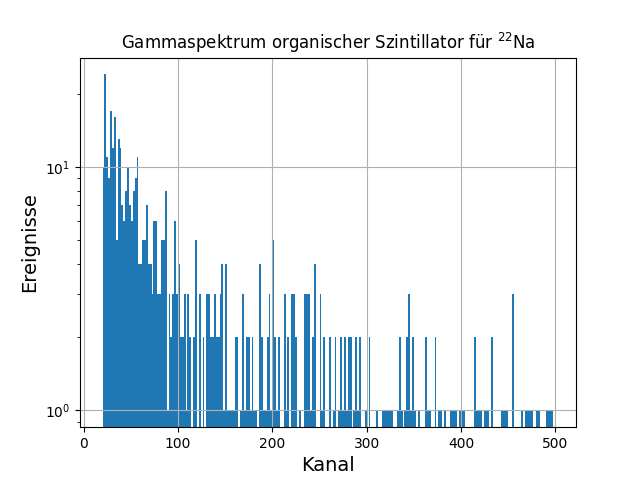
\includegraphics[width=\linewidth]{images/Na22szin.png}
  \caption{Szintillator}
  \label{NaSzin}
\endminipage\hfill
\end{figure}

Die $^{133}$Ba Probe besaß eine im Vergleich dazu deutlich stärkere Aktivität, was sich positiv auf die Spektren (\ref{BaGe} und \ref{BaSzin}) ausgewirkt hat.
Im Spektrum des Ge-Detektors lassen sich jetzt mehrere Peaks deutlich erkennen.
Eine Kalibirierung anhand dieser sollte jetzt möglich sein.
Das Szintillator Spektrum dieser Probe wird, wie  zu erwarten war, vom Compton-Kontinuum dominiert.
Die Compton-Kante ist hierbei schwach ausgeprägt, was eine herkömliche Kalbirierung, wieder wie zu erwarten, erschweren würde.
Eine längere Messzeit oder Beseitigung der Untergrundstrahlung, würde hier jedoch möglicherweise aushelfen können.
Aufällig ist außerdem ein recht stark ausgeprägter Peak im niedrigenergetischen Bereich (ungefähr bei Kanal 50).
Hierbei könnte es sich um einen stark ausgeprägten Rückstreupeak handeln.
Aufgrund der besseren Spektren, wird im folgenden die $^{133}$Ba Probe genutzt.

\begin{figure}[h]
\minipage{0.5\textwidth}
  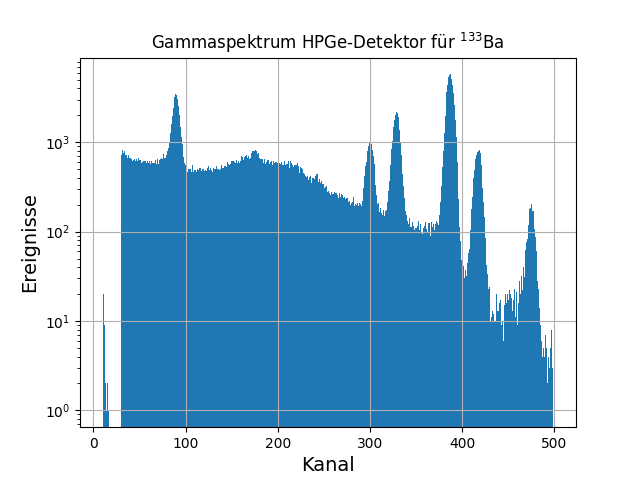
\includegraphics[width=\linewidth]{images/ba133Ge.png}
  \caption{Ge-Detektor}
  \label{BaGe}
\endminipage\hfill
\minipage{0.5\textwidth}
  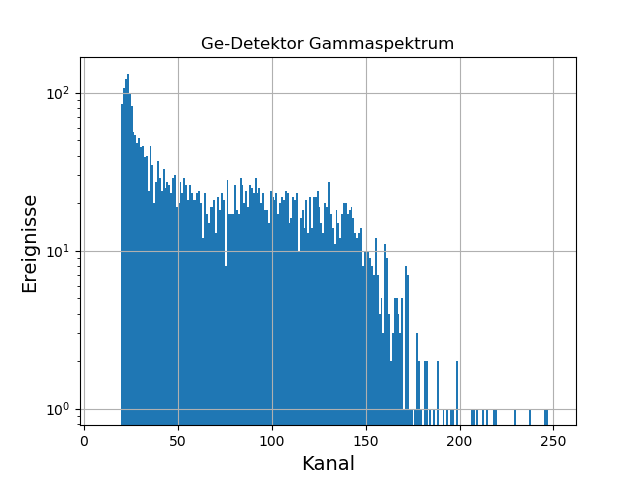
\includegraphics[width=\linewidth]{images/ba133Szin.png}
  \caption{Szintillator}
  \label{BaSzin}
\endminipage\hfill
\end{figure}

\subsection{Energiekalibrierung des Ge-Detektors}

Ausgehend vom aufgenommenen Spektrum wird im folgenden eine Energiekalibrierung des Ge-Detektors mitels einer Vollenergiepeak-Analyse durchgeführt.
Dafür ist es als erstes notwendig die sichtbaren Peaks zu identifizieren.
Dies wurde durch vergleiche mit bekannten Nuklid-Karten (Quelle iaea einfügen) realisiert.
Die Ergebnisse sind in Abb. \ref{GeKali} zu sehen.
Eine Identifikation der Peaks, mit den zu häufigsten Gammazerfällen von $^{133}$Ba war möglich.
Zusätzlich zu diesen, fällt jedoch ein weiterer Peak, mit relativ geringer Intensität, um Kanal 480 herum auf.
Ein entsprechender Gammazerfall von $^{133}$Ba ist nicht in (Quelle iaea einfügen) zu finden.
Daher sollte es sich hier um Untergrundstrahlung von einem natürlichen Nuklid handeln.
Eine identifkation von diesem könnte erfolgen, aufgrund der relativ geringen Intensität und der foldendermaßen hohen statistischen Ungenauigkeit, wurde dies jedoch nicht getan und der Peak nicht für die kalibrierung genutzt.

\begin{figure}[h]
  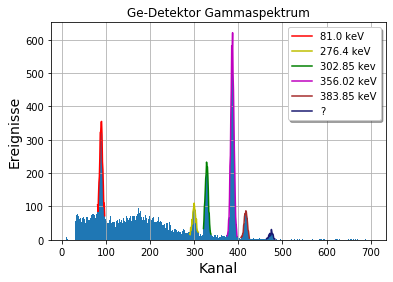
\includegraphics[width=\linewidth]{images/ba133Kali.png}
  \caption{Vollenergiepeakanalyse des Ge-Detektors mit $^{133}$Ba Spektrum}
  \label{GeKali}
\end{figure}

Die entsprechenden Peaks wurden mit einer Gaussfunktion entsprechend
\begin{equation}
N(K) = a \cdot exp \left( - \frac{(K - K_{0}^{2}}{2 \sigma ^{2}} \right)
\end{equation}


gefittet um Mittelwerte ($\mu$) und Standardabweichungen {$\sigma$} dieser zu bestimmen.
In der Gaussfunktion dient $a$ als Normierungsfaktor, der für die weitere Betrachtung keine Rolle spielt.
Die Ergebnisse sind in Tabelle \ref{peaks} zusammengefasst.
Hier fällt auf, dass die Standardabweichungen der Peaks recht konstant sind.

\begin{table}[h]
\centering
\begin{tabular}{|c | c |c |}
\hline
$E_{\gamma}$ [\si{\kilo\electronvolt}]  & $\mu$ & $\sigma$ \\
\hline
81.00 & 89.0 & 3.1 \\
276.40 & 299.9 & 3.6 \\
302.89 & 328.4 & 3.7 \\
356.02 & 386.4 & 3.7 \\
383.85 & 416.8 & 3.7 \\
\hline
\end{tabular}
\caption{Gaussfit der Peaks}
\label{peaks}
\end{table}

Aus den Mittelwerten wird der Kanal, welcher mit der Zerfallsenergie korrespondiert, bestimmt, indem der Mittelwert ($\mu$) zur nächsten natürlichen Zahl K gerundet wird.
Als Maß für die Unsicherheit der Energiebestimmung, wird die mittlere Halbwertsbreite (FWHM), ebenfalls auf natürliche Zahlen gerundet, genutzt.
Diese ist defininiert, als Breite der Gaussfunktion bei halber Höhe und dient uns als Unsicherheit der Energiebestimmung.
Sie berechnet sich aus der Standardabweichung ($\sigma$) mit:
\begin{equation}
FWHM = 2 \sqrt{2 ln2} \sigma
\end{equation}

Die Ergebnisse sind in Tab. \ref{kanal} zusammengefasst.

\begin{table}[h]
\centering
\begin{tabular}{|c | c |c |}
\hline
$E_{\gamma}$ [\si{\kilo\electronvolt}]  & $K_{\gamma}$ & FWHM \\
\hline
81.00 & 89 & 7 \\
276.40 & 300 & 8 \\
302.89 & 328 & 9 \\
356.02 & 386 & 9 \\
383.85 & 417 & 9 \\
\hline
\end{tabular}
\caption{Bestimmung der Kanäle}
\label{kanal}
\end{table}

Mit Kentnis der Fünf Energiepeaks sowie der korrespondierenden Kanäle ist jetzt die Bestimmung einer Kalibriergerade des Ge-Detektors möglich.
Dafür wurden die Energien über die Kanäle geplottet und eine lineare Regression vorgenommen.
Das Ergebnis dieser ist in \ref{Gegerade} zu sehen.
Als Regressionsparameter ergaben sich ein Anstieg von: $n = 0.924 \pm 0.002$ sowie ein Schnittpunkt von $m = -1.1 \pm 0.7$.
Die Ungenauigkeiten ergeben sich hierbei aus der Regression.
Damit ergibt sich die Kalibriergerade des Ge-Detektors zu:
\begin{equation}
E(K) = (0.924 \cdot K - 1.1) \ \si{\kilo\electronvolt}
\end{equation}
Ausgehend von den Ungenauigkeiten der Regressionsparameter, lässt sich eine Ungenauigkeit der Energie mithilfe der Fehlerfortpflanzung bestimmen.
Damit ergibt sich für jeden Kanal K eine Ungenauigkeit der Energie von:
\begin{equation}
\sigma E(K) = \sqrt{4 \cdot 10^{-6} K^2 + 0.49} \ \si{\kilo\electronvolt}
\end{equation}
Im betrachteten Energiebereich von bis zu einigen hundert \si{\kilo\electronvolt}, entspricht dies ungefähr einer Abweichung von $0.7 \ \si{\kilo\electronvolt}$ für jeden Kanal.

Dabei ist zu beachten, dass dies in erster Linie eine numerische Ungenaugkeit aus der Regression ist.
Physikalische oder technische Ungenauigkeiten, wie z. B. die Untergrundstrahlung, wurden hier nicht betrachtet.

\begin{figure}[h!]
  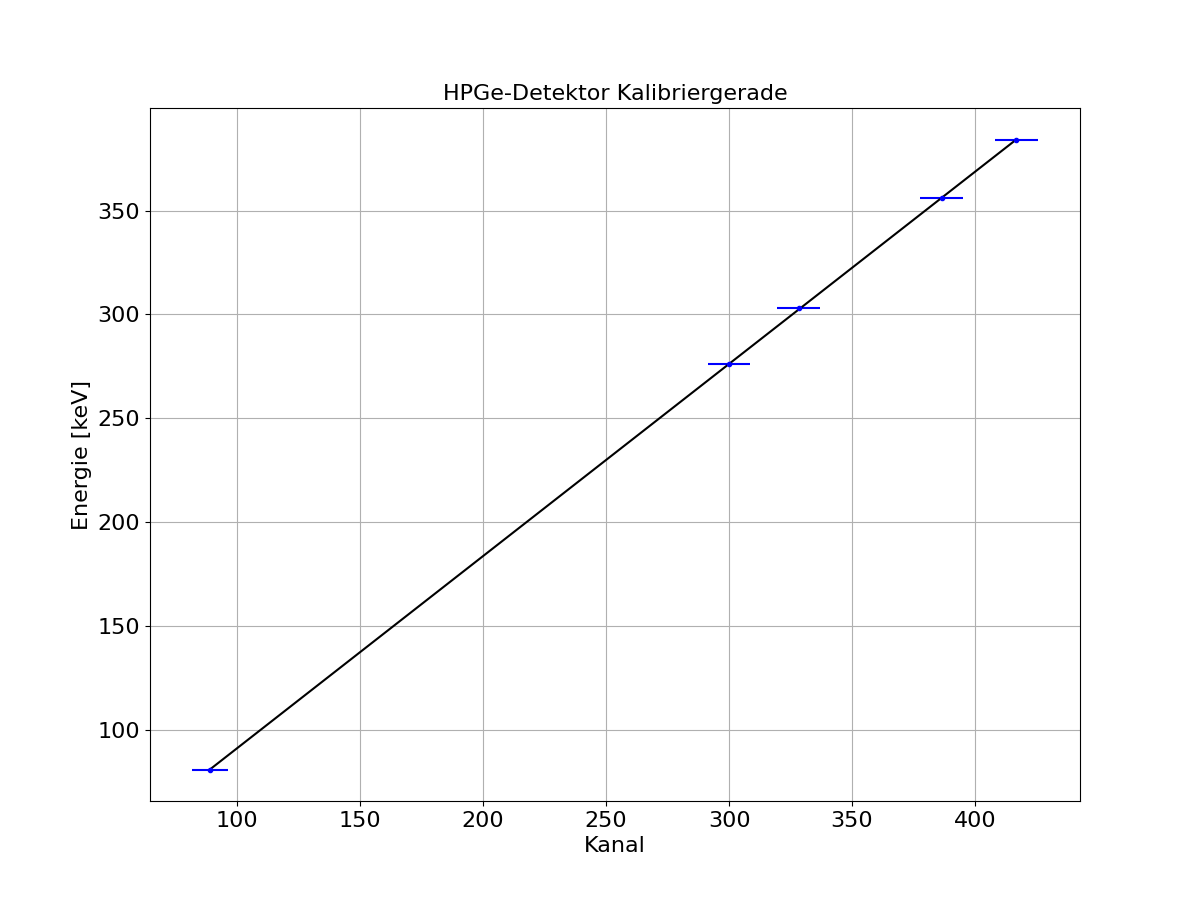
\includegraphics[width=\linewidth]{images/Kalibriergerade1.png}
  \caption{Kalibriergerade des Ge-Detektors}
  \label{Gegerade}
\end{figure}
